The purpose of this section is to deliver a broad understanding of what Identity Management Provisioning (IMP) is, what an IMP service can look like and how identity management provisioning systems can operate.

\subsection{IMP}
Identity Management Provisioning is a method where identity management is provided as a service to users and Service Providers. The service enables users to create and manage a digital identity and use it to share personal information and interact with Service Providers.

Many identity management systems currently in use by Service Providers require the user to create a new user profile, specify login credentials and keep the personal Information up to date. Every Service Provider operates their own identity management system and users have to access each system individually through multiple websites to use their user profiles. This approach to identity management leads to several problems which are discussed in section \ref{section:identity_management_issues}.

In contrast to a user profile based identity management approach, IMP provides identity management as a service. Only one identity management provisioning system is hosted and accessed by users and Service Providers. Users therefore only need one IMP identity, which is accessed by multiple Service Providers. This approach to identity management is capable of solving various issues of user profile based identity management that are discussed in section \ref{section:imp_solution_opportunities}

To access the IMP service, users can use applications or websites. Service Providers however often require integration into their existing system architecture to enable existing system components to use the new identity management method.

\subsection{IMP Service}

There are many ways to design a service for identity management provisioning. This section describes what an identity management provisioning service can look like. The content of this section is based on the IMP service provided by IDAS \cite{idas}.

Software tools exist for users and Service Provider to access the IMP service. 
For the user, this is a smartphone application. For the Service Provider this is an integration component. The smartphone application provides a user friendly graphical interface which enables the user to receive notifications, maintain personal information, share personal information, and more. The integration component for the Service Provider is a software solution with similar capabilities as the smartphone app but designed towards enterprise use. It therefore has no graphical user interface but additional business relevant features and integration capabilities. IMP application and integration component are described in section \ref{section:imp_system} in more detail.

One important part of the IMP service is management of personal information by users. After installation of the smartphone application, a new identity (IMP identity) can be created. As part of this identity, the user can add any amount of key-value pairs as attributes, the list of all attributes making up the personal information of the IMP identity. Despite being able to add any key-value pair, there are some commonly used keys like name, age, home address etc. Depending on the use case of Service Providers, multiple more keys and their meaning have to be agreed upon. This means the IMP service has to define a canonical data model. Each Service Provider then translates it to their individual data models.

Many Service Providers require users to manually verify their identity and personal information by for example visiting a store and showing their ID card. Similar verification processes are expected to be used by the IMP service to verify IMP identities and their personal information. However, for simplification reasons, the details of this verification process are left out .

Users and Service Providers can establish relationships and use them to share personal information and interact. The initial form of a relationship is a relationship template, which is created by the Service Provider and describes what types of relationships they are willing to establish. The templates are made available to interested users, which can use them to request relationships.

A Service Provider fill a relationship template with optional and mandatory information:

\paragraph{Title} The title describes the purpose of the relationship in a short way. 
    
\paragraph{Requested Attributes} The Service Provider can list keys of attributes he requires the user to share in order to send a relationship request. When the user submits a relationship request based on this relationship template, the values filled in for the requested attributes are copied and sent as part of the request. The recipient of the request can use the personal information to decide whether to accept or reject the relationship.
    
\paragraph{Shared Attributes} Shared Attributes is a list of key-values pairs that the Service Provider makes available to any user interested in requesting a relationship. The Service Provider has to share a minimal amount of attributes that enable the user to identify it. 
    
\paragraph{Purpose} This is a text field where the Service Provider can give a detailed explanation of what the purpose of the relationship is, e.g what effects a relationship request and an established relationship will have. The reason for why the requested attributes are necessary for the relationship have to be explained here as well as how each shared attribute is going to be processed. This helps the user in making an informed decision on whether to submit the relationship request or not.
    
\paragraph{Attachments} Attachments can be all kinds of documents and files. For example legal information can be included but also product flyers corresponding to the relationship template, etc.
    
\paragraph{Metadata} Metadata can be any type of information which should not be displayed to the user but is necessary for the user application or the Service Provider to process the relationship process.

When the user receives the template through his IMP application, the requested attributes are automatically filled in if they exist for his IMP identity. Otherwise they can be filled in manually and added as new attributes of the IMP identity.

At this point it is important to take a look at how IMP identity attributes and shared attributes are separated. IMP identity attributes are managed by the user to reflect the most up to date information. Attributes shared as part of a relationship can be automatically filled with values from the IMP identity but can also be manually entered. This means, shared attributes and IMP identity attributes are not necessarily the same. 

Based on the information about the Service Provider and the purpose of the relationship, the user can decide to send a relationship request or not. If the user decides to request the relationship, the request is sent to the Service Provider. If the Service Provider approves the request, the relationship is established and both parties get notified. Through the IMP application, the user can see all relationships as well as their status, the content of the underlying relationship template and a list of shared attributes and their values.

As part of an established relationship, user and Service Provider can interact with each other by asynchronously exchanging structured data packages as IMP messages. IMP messages can contain any content, however, both IMP application and Service Provider systems should be able to understand the messages. For this purpose, besides content, messages are expected to contain some identification value like a message type. The integration component provided to the SP does not process the content of messages but simply makes the messages accessible to the system architecture of the Service Provider. Without additional integration systems, the Service Provider has to implement his own solutions for understanding and processing messages. The IMP application however, has a set of messages it understands. The list of messages the application is able to process can be expanded by the identity management provider who develops it.

Some important messages the IMP application understands and the Service Provider should be able to process are:

\paragraph{Mail} Messages of the mail type can be used by Service Provider and user to exchange human readable text. Mails sent to an IMP identity are displayed by the IMP application through for example a notification. 
The IMP application defines a format for the content of the mail. The term "mail" is used as an alternative to the term "message", as messages will later be used in context of a messaging system.

\paragraph{Attribute Change} Messages of the attribute change type can be used by the user to request the modification of shared attributes. The user can modify, add or delete attributes shared as part of a relationship and submit an attribute change request to the Service Provider which contains the changes. The Service Provider can decide to either accept or reject the request and respond with a corresponding attribute change response message. 
The IMP application defines a format for the content of the attribute change request and response messages.

\paragraph{Authentication} Messages of the authentication type can be used by the Service Provider to request confirmation from the IMP identity for specific business process. The Service Provider sends an initial request message to the IMP identity which contains a description of what confirmation is requested by the user. Through the IMP application the user is notified and can accept or reject. Depending on the interaction by the user, the IMP application sends a response message to the Service Provider. 
The IMP application defines a format for the content of the authentication request and response messages.

The IMP system guarantees that all information is encrypted and can only be deciphered by identities that are allowed to read it. This usually does not include the systems hosting the IMP service. Only the owner of an identity can manage attributes of their identity. A relationship is established only with the identity presented as part of the relationship request and only the specified attributes are shared. Interactions as part of a relationship are only possible between the two parties of the relationship and cannot be intercepted or modified by others.

\subsection{IMP System} \label{section:imp_system}
This section describes the IMP system which is the system architecture required for providing the IMP service described in the previous section. The content of this section is based on the IMP system used by IDAS \cite{idas}.

\begin{figure}[h!]
    \centering
    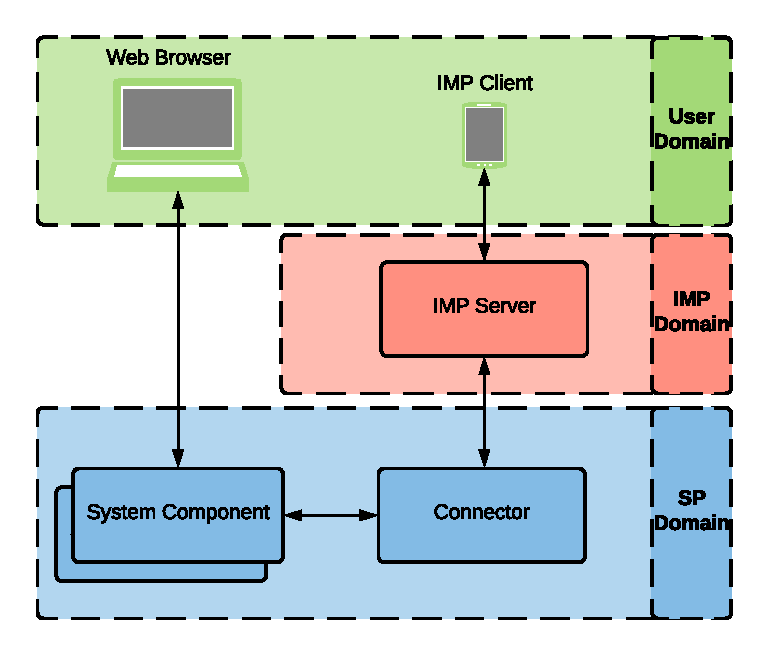
\includegraphics[scale=0.6]{Diagrams/IMP System Overview.pdf}
    \caption{IMP System Overview}
    \label{imp:imp_system_overview}
\end{figure}

As shown in figure \ref{imp:imp_system_overview}, the IMP system can be separated into three domains. \\
The user domain contains systems that the user directly interacts with. These typically are applications on PC or smartphone and websites. IMP application on smartphones are provided to users for accessing IMP services. For simplification, each user is assumed to access the IMP service through one device which eliminates the need for device synchronization. As previously described, the IMP application enables the user to manage attributes of their identity, to establish relationships, to manage relationships and to interact with messages through relationships. 

The Service Provider domain contains the system architecture of the Service Provider and the IMP connector. The IMP connector contains a REST API which enables the system architecture to access IMP services.

The IMP domain contains all identity management provisioning systems required to be hosted by the identity management provider. In this case, the domain contains only the IMP server. The IMP server is able to communicate with each IMP application and IMP connector. It has the purpose of maintaining a - when necessary encrypted - list of all identities, relationships, relationship templates and IMP messages. As the IMP server does not know the private key corresponding to the IMP identity, it is unable to decipher the data. The IMP server is also capable of creating relationship templates, processing and routing relationship requests and responses and IMP messages. The exact details of how the IMP server operates is too broad to be covered in this thesis.

\begin{figure}[h!]
    \centering
    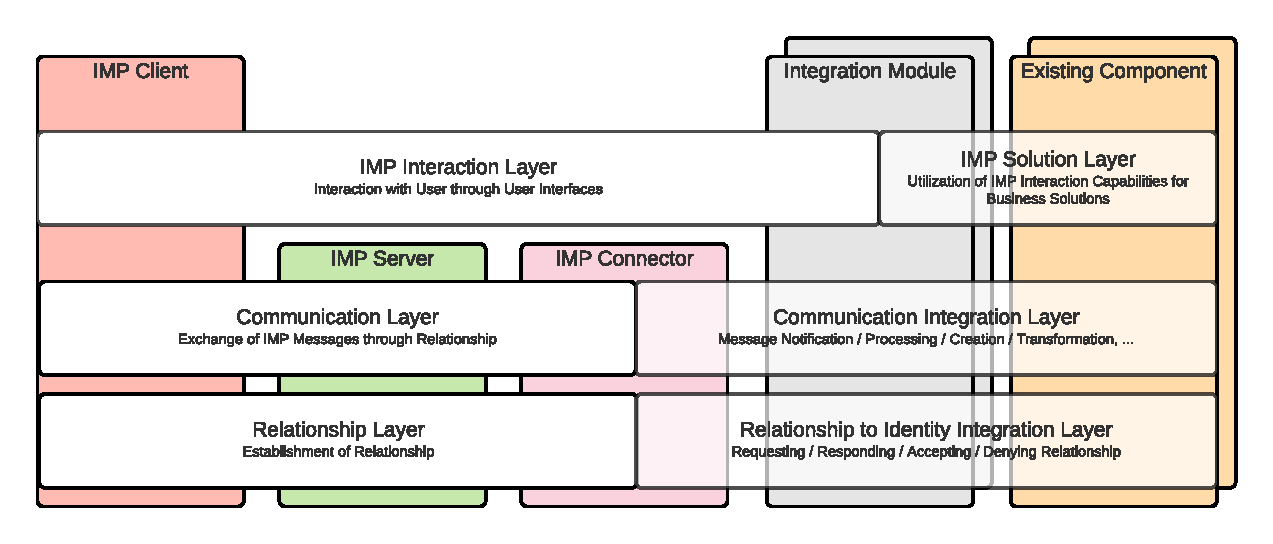
\includegraphics[scale=0.6]{Diagrams/IMP Layer Diagram.pdf}
    \caption{IMP System Operation Layers}
    \label{imp:layer_diagram}
\end{figure}

As shown in figure \ref{imp:layer_diagram}, the operation of IMP systems can be separated into multiple layers. The layers build upon each other (from bottom to top) and provide an increasingly abstract perspective on the functionalities of each component. 

The vertical bars in the figure represent all previously described components of the IMP system and one additional component called "Integration Module". The "Integration Module" is not important at the moment and will be the focus of following chapters. The horizontal bars in the figure represent layers of IMP system operation. From bottom to top, the layers describe the operation of the IMP system increasingly more abstract from the underlying technology. In addition to that, each bar is split up into two sides, however, in this section only the left side is relevant.

The lowest layer is called "Relationship Layer". On this layer, the IMP system operates by establishing relationships. IMP application and IMP connector exchange relationship requests and responses through the IMP server in order to establish new relationships. The IMP server maintains a list of all relationships and their status.

Once a relationship is established, the IMP system operates on the "Communication Layer". On this layer, IMP messages are exchanged as part of an active IMP relationship between IMP application and IMP connector. The application can create, send, receive, process and display a list of IMP messages that it is able to understand. The IMP connector is able to send and receive IMP messages through a relationship without requiring to know details about the content. The IMP server stores an encrypted backup of all messages.

Using IMP relationships and IMP messages, the Service Provider can interact with the user on the "IMP Interaction Layer". On this layer, depending on the use case, different purposes can be assigned to interaction possibilities. For example, a Service Provider can decide to use relationships as a way to receive product or subscription orders. Another possibility would be to use relationships for filling in a form as part of a survey.

\subsection{IMP Use Cases}

In this section the IMP system operation for the most important use cases of the IMP service are described in more detail.

\subsubsection{Establish Relationship}

This section elaborates the sequence of establishing an IMP relationship as shown in figure \ref{imp:establish_relationship}.
The first step towards a relationship is the interest of a user. A user for example wants to subscribe to the newsletter of a Service Provider. The Service Provider needs personal information of the users to be able to send them personalized mails. To obtain the necessary attributes and receive the approval of the users, the Service Provider requires  established relationships.

\begin{figure}[h!]
    \centering
    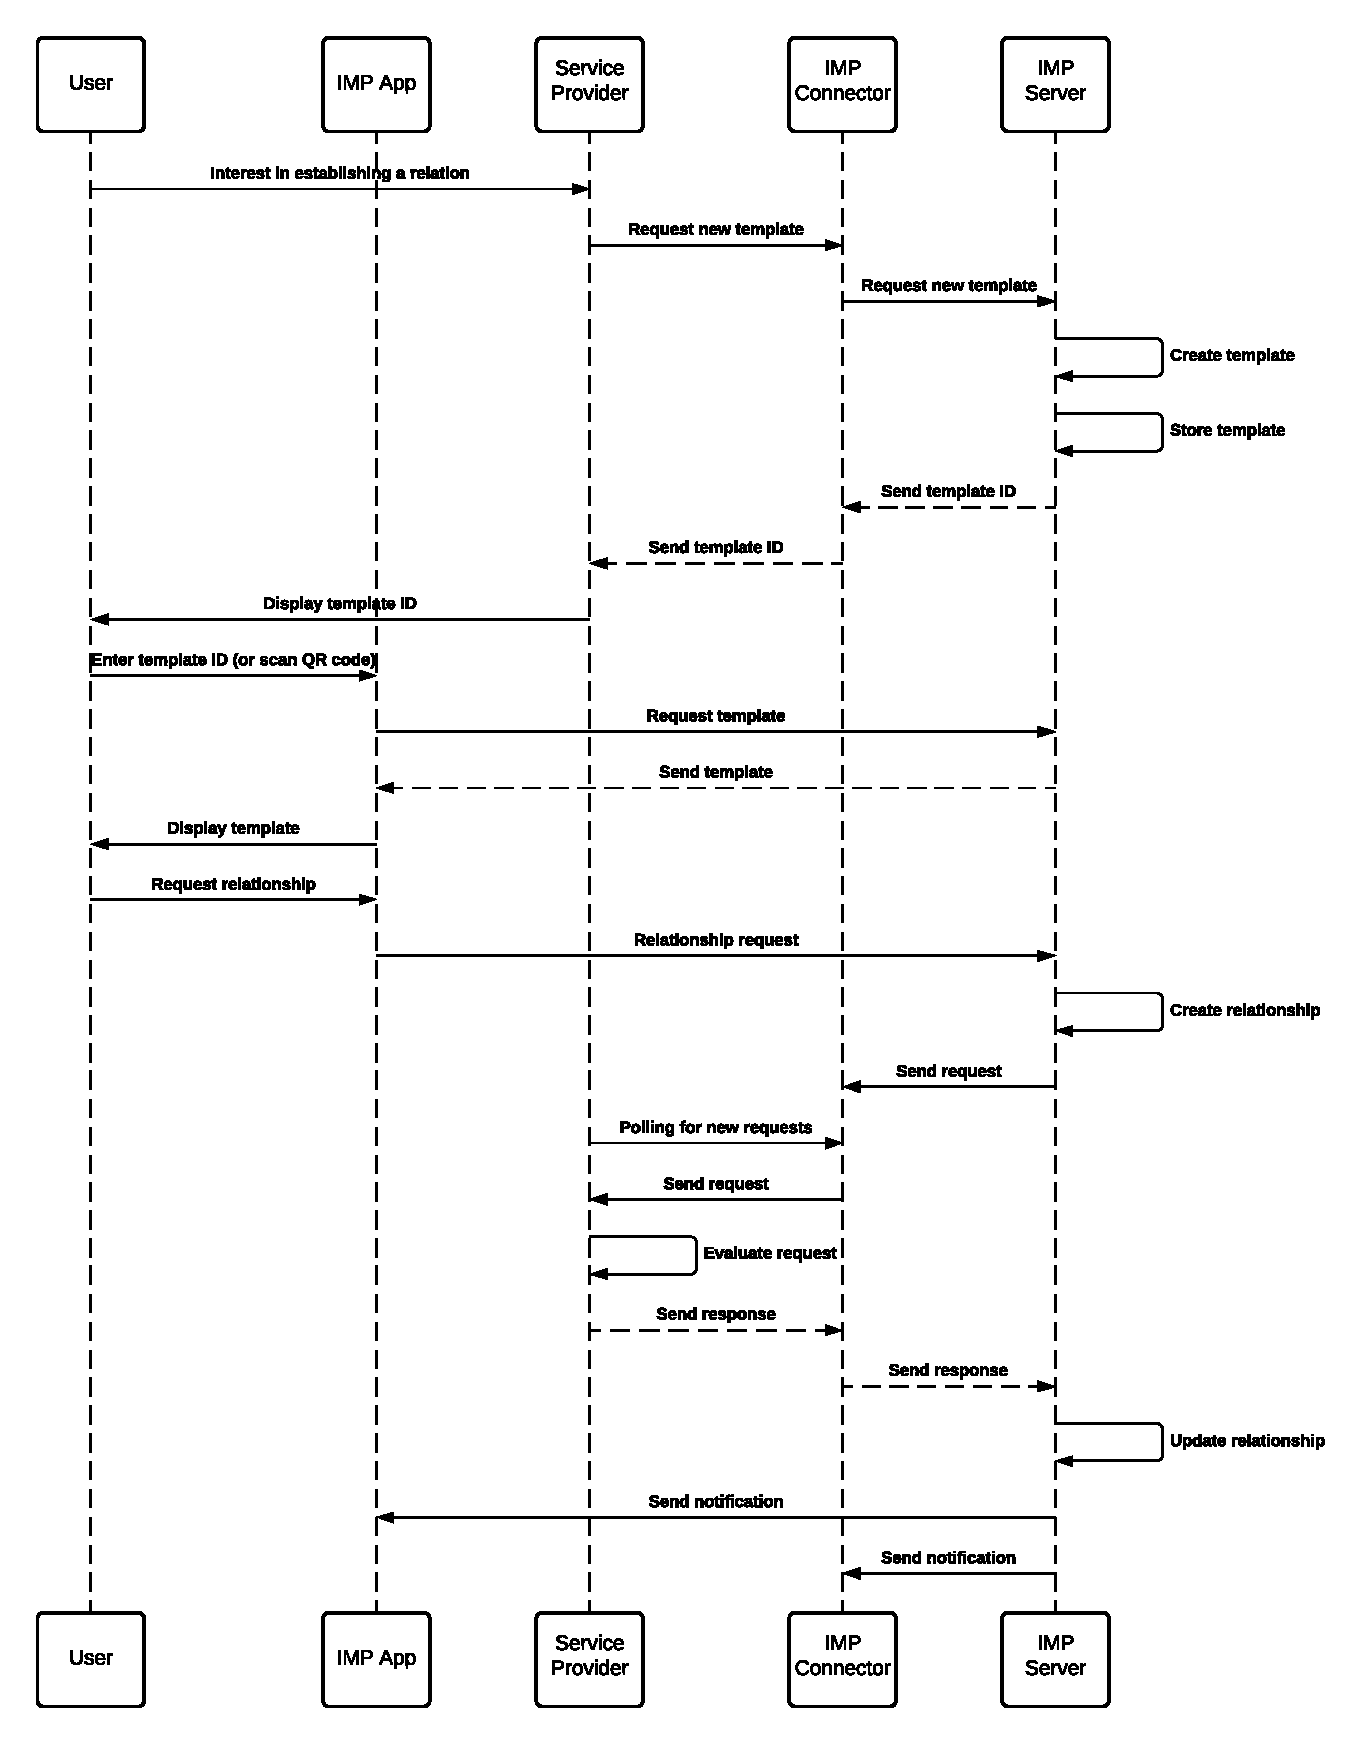
\includegraphics[scale=0.6]{Diagrams/IMP Use Case Establish Relationship Sequence Diagram.pdf}
    \caption{Establish Relationship Sequence Diagram}
    \label{imp:establish_relationship}
\end{figure}

To enable users to request a relationship with the purpose of subscribing to a newsletter, the Service Provider has to create a relationship template. Through the REST interface of the connector, the SP sends a request for a new relationship template. The request contains parameters specifying the content of the relationship template. In this case, the relationship template could be configured as follows:
\begin{figure}[h!]
    \begin{itemize}
    \item Title: Subscribe to the newsletter
    \item Requested Attributes: Name, Surname, E-Mail address, Interests
    \item Shared Attributes: SP Name, SP address, SP phone number, SP E-Mail address
    \item Purpose: By accepting this relationship, you agree to receive personalized emails to the shared address. Name, surname and interests are required to personalize the content of the emails.
    \item Attachments: required legal document
\end{itemize}
\end{figure}


Based on the parameters of the request, the connector creates a relationship template and sends it to the IMP server. The server stores the template and returns a relationship template ID. Through this ID, the corresponding template can be retrieved from the IMP server.
The Service Provider can transmit the template ID to any user who wishes to subscribe to a newsletter. This can be done by for example rendering the template ID as a QR code on a website.
If the QR code is displayed to the user, he can scan it using the IMP application. The application understands that the content of the QR code contains a relationship template ID and retrieves the corresponding template from the IMP server.

The IMP application displays the relationship template to the user and automatically fills in as many requested attributes as possible.

The user can now decide if he wants to accept the relationship and share the requested attributes. If he accepts, IMP application sends a relationship request to the IMP server. The request contains all information of the relationship template in addition to the shared attributes of the user.

Based on the relationship request, the IMP server creates a relationship with the status "pending". A unique relationship ID is attached. The server then forwards the relationship request to the connector of the Service Provider.

As the system architecture of the Service Provider has no way of knowing when the connector receives a relationship request, he iteratively requests an update from the connector through its REST interface. The connector responds with the received relationship request, provided a request was submitted. The system architecture of the Service Provider processes the request in order to decide if it should be accepted. The Service Provider could for example verify if a relationship with the identity already exists or if the e-mail address is already registered.

The system architecture sends a relationship response to the REST interface of the connector. The response contains all information of the received relationship request with optional additional information the Service Provider might want to share now. This could for example be the name of the newsletter the Service Provider decided to select for the user based on his specified interests.

The connector sends the relationship response to the IMP server which updates the content and status of the corresponding relationship. It might be possible that the user retracted the relationship request in the meantime. In this case, the relationship response would be dropped by the IMP server and the connector would be notified.
If however, the IMP server updates the status of the relationship to "established", both IMP application and connector are notified with the final content of the relationship.

After receiving the final "relationship established" notification, the system architecture of the Service Provider can store the shared attributes in a database along with the corresponding relationship ID.

\subsubsection{Attribute Change}
This section describes the sequence of changing an attribute shared as part of an IMP relationship as shown in figure \ref{imp:attribute_change}. If the user switches to a new e-mail provider, he will need to change the corresponding e-mail attribute shared as part of the relationship to receive the newsletter on his new e-mail address.

\begin{figure}[h!]
    \centering
    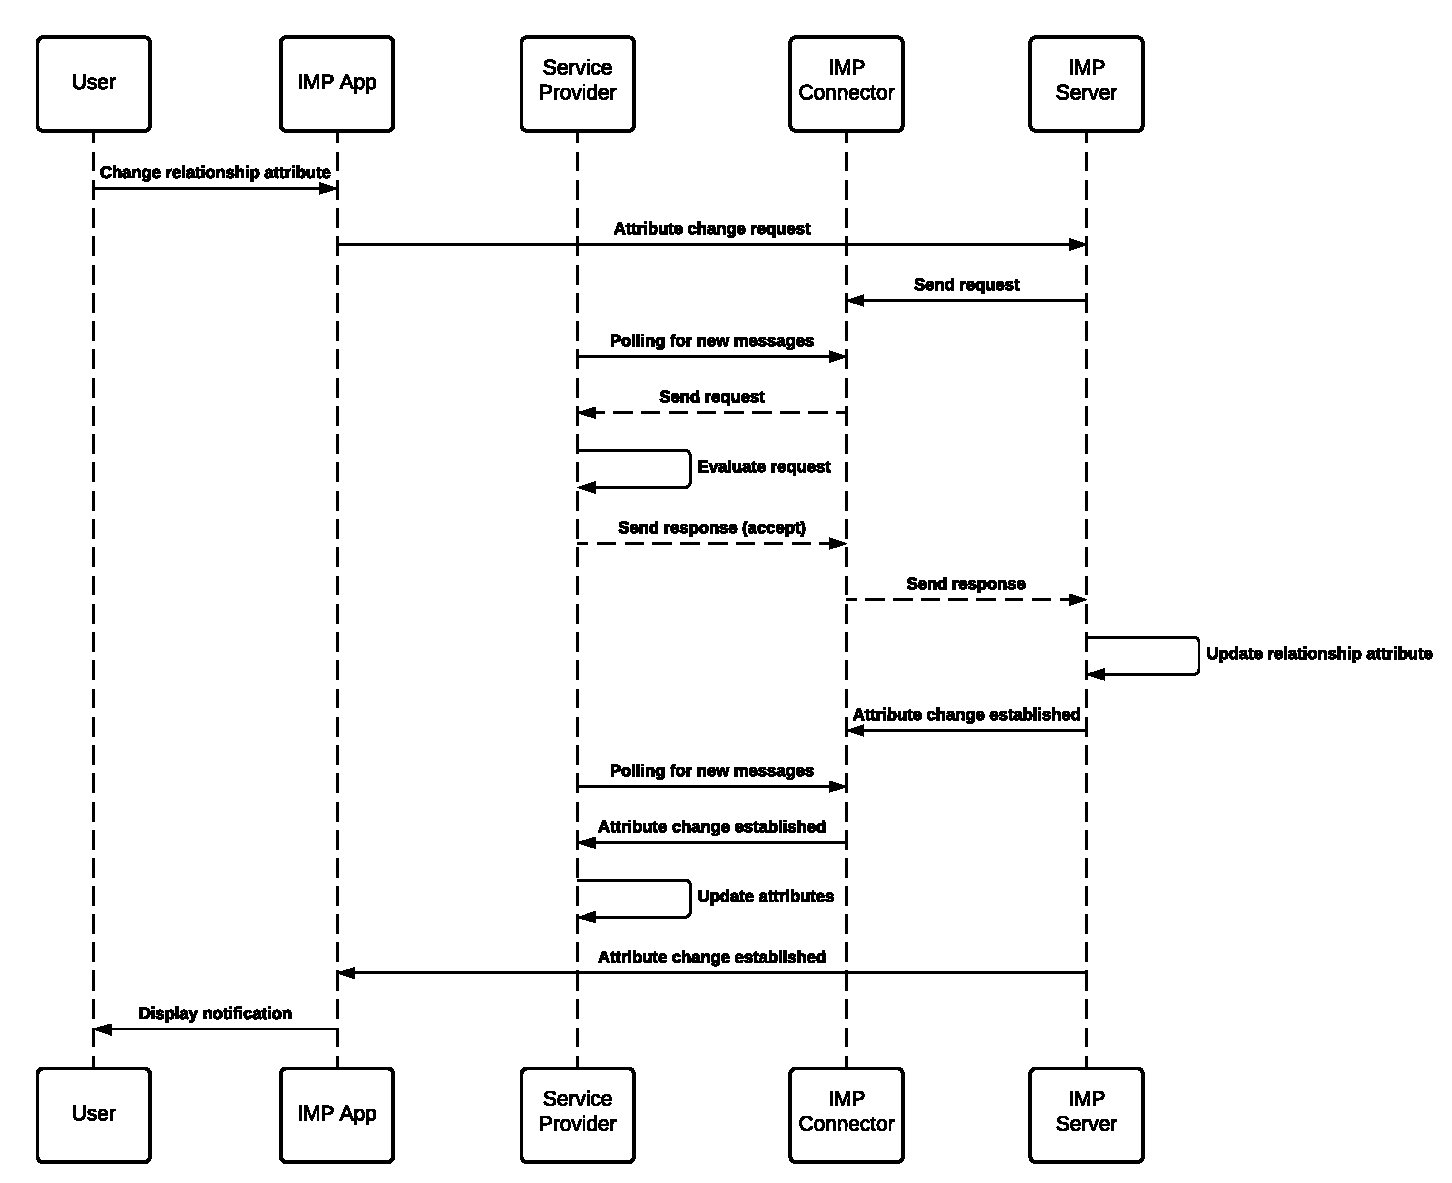
\includegraphics[scale=0.6]{Diagrams/IMP Use Case Change Realtionship Attribute Sequence Diagram.pdf}
    \caption{Change Relationship Attributes Sequence Diagram}
    \label{imp:attribute_change}
\end{figure}

Through the IMP application, the user can view relationships and edit shared attributes. After changing an attribute, for example the e-mail address, the IMP application sends an attribute change request to the IMP server, which forwards it to the IMP connector corresponding to the IMP relationship. Through the REST interface of the IMP connector, the Service Provider regularly polls for new messages and eventually receives the attribute change request. The Service Provider evaluates whether to accept or reject the request and uses the REST interface of the IMP connector to submit the response. The IMP connector sends the response to the IMP server which - if the Service Provider accepted the request - notifies IMP connector and IMP application of the successful change of attributes. The Service Provider again polls for new messages and eventually receives the attribute change established notification based on which it now updates the stored attributes associated to the relationship. When the IMP application receives the attribute change established message, it displays a notification to the user.

\subsubsection{Mail}
This section elaborates the sequence of sending a mail as part of an IMP relationship as shown in figure \ref{imp:mail}.
If a user for example has questions about the newsletter, he can send a mail to the Service Provider as part of the established relationship.

\begin{figure}[h!]
    \centering
    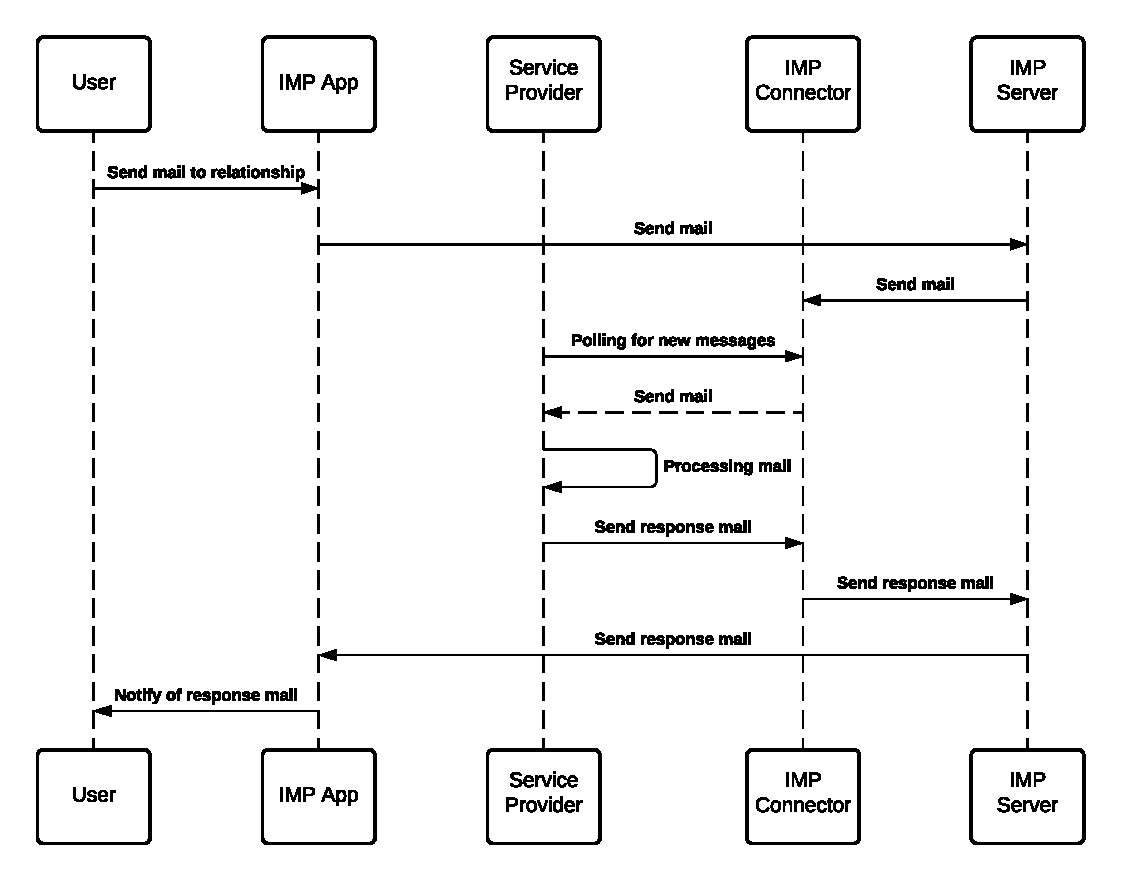
\includegraphics[scale=0.6]{Diagrams/IMP Use Case Mail Sequence Diagram.pdf}
    \caption{Mail Sequence Diagram}
    \label{imp:mail}
\end{figure}

Through the IMP application the user can view relationships and submit mails. Once submitted, the IMP application sends the mail to the IMP server which forwards it to the IMP connector corresponding to the relationship. The Service Provider polls for new messages and eventually receives the mail as response. An employee of the Service Provider can process the email and use the REST interface of the IMP connector to send a response mail to the same relationship. The IMP connector sends the mail to the IMP server which forwards it to the IMP application of the IMP identity corresponding to the IMP relationship. The application then notifies the user of the received mail.

\subsubsection{Authenticate}
This section elaborates the sequence of authenticating as part of an IMP relationship as shown in figure \ref{imp:authenticate}.
If the Service Provider wants to request confirmation from the user, they can send an authentication request to the corresponding relationship.

\begin{figure}[h!]
    \centering
    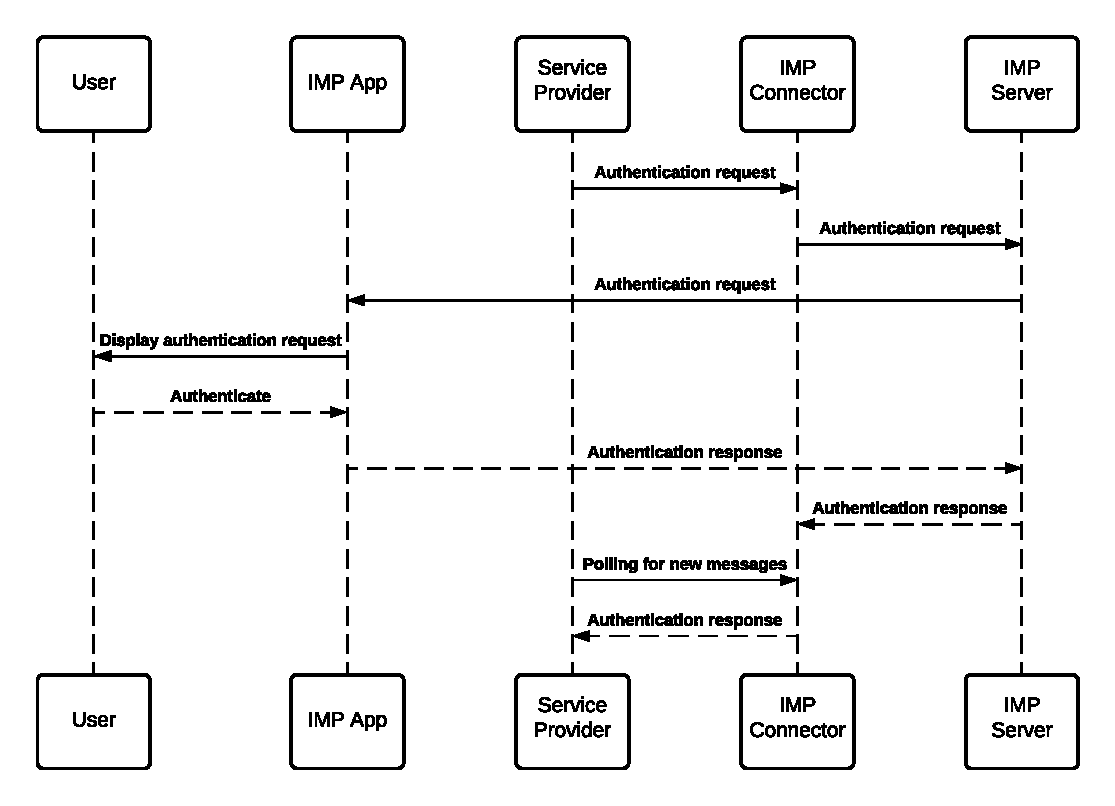
\includegraphics[scale=0.6]{Diagrams/IMP Use Case Authenticate Sequence Diagram.pdf}
    \caption{Authenticate Sequence Diagram}
    \label{imp:authenticate}
\end{figure}

The SP uses the REST interface of the IMP connector to send an authentication request as part of an IMP relationship. The IMP connector sends the request to the IMP server which forwards it to the IMP application of the IMP identity corresponding to the IMP relationship. The application displays the authentication request to the user. The user can accept or reject the request which will result in the corresponding authentication response by the IMP application. The response is sent to the IMP server which forwards it to the IMP connector corresponding to the IMP relationship. The Service Provider polls for new messages and eventually receives the authentication response.